%    Copyright (c)  2024  João Augusto Costa Branco Marado Torres.
%    Permission is granted to copy, distribute and/or modify this document
%    under the terms of the GNU Free Documentation License, Version 1.3
%    or any later version published by the Free Software Foundation;
%    with no Invariant Sections, no Front-Cover Texts, and no Back-Cover Texts.
%    A copy of the license is included in the section entitled "GNU
%    Free Documentation License".
%
%    You should have received a copy of the GNU Free Documentation License
%    along with this program.  If not, see <https://www.gnu.org/licenses/>

%%%%%%%%%%%%%%%%%%%%%%%%%%%%% Define Article %%%%%%%%%%%%%%%%%%%%%%%%%%%%%%%%%%
\documentclass[a4paper,12pt]{article}
%%%%%%%%%%%%%%%%%%%%%%%%%%%%%%%%%%%%%%%%%%%%%%%%%%%%%%%%%%%%%%%%%%%%%%%%%%%%%%%

%%%%%%%%%%%%%%%%%%%%%%%%%%%%% Using Packages %%%%%%%%%%%%%%%%%%%%%%%%%%%%%%%%%%
\usepackage{geometry}
\usepackage{graphicx}
\usepackage{amssymb}
\usepackage{amsmath}
\usepackage{amsthm}
\usepackage{empheq}
\usepackage{mdframed}
\usepackage{booktabs}
\usepackage{lipsum}
\usepackage{graphicx}
\usepackage{color}
\usepackage{psfrag}
\usepackage{pgfplots}
\pgfplotsset{compat=1.18}
\usepackage{bm}
% % % % % % % % % % % % % % % % % % % % % % % % % % % % % % % % % % % % % % % %
\usepackage[utf8]{inputenc}
\usepackage[english]{babel}
\selectlanguage{english}
\usepackage{blindtext}
\usepackage{csquotes}
\usepackage{hyperref}
\hypersetup{colorlinks,
           %citecolor=black,
           %filecolor=black,
           %linkcolor=black,
           %urlcolor=black,
           bookmarksopen=true}
\usepackage[
backend=biber,
style=alphabetic,
sorting=ynt
]{biblatex}
\addbibresource{references.bib}
\usepackage{bookmark}
\usepackage{enumitem}
\usepackage{fancyhdr}
\pagestyle{fancy}
\fancyfoot[C]{\copyrightnotice}
\setlength{\headheight}{14.5pt}
%\addtolength{\topmargin}{-2.5pt}
\usepackage{mathtools}
\usepackage{tikz}
\usetikzlibrary{positioning,fit,calc}
\usepackage{float}
\usepackage{wrapfig}
%%%%%%%%%%%%%%%%%%%%%%%%%%%%%%%%%%%%%%%%%%%%%%%%%%%%%%%%%%%%%%%%%%%%%%%%%%%%%%%

% Other Settings

\pagenumbering{arabic}
\hfuzz = .6pt % avoid black boxes

%%%%%%%%%%%%%%%%%%%%%%%%%% Page Setting %%%%%%%%%%%%%%%%%%%%%%%%%%%%%%%%%%%%%%%
\geometry{a4paper}

%%%%%%%%%%%%%%%%%%%%%%%%%% Define some useful colors %%%%%%%%%%%%%%%%%%%%%%%%%%
\definecolor{ocre}{RGB}{243,102,25}
\definecolor{mygray}{RGB}{243,243,244}
\definecolor{deepGreen}{RGB}{26,111,0}
\definecolor{shallowGreen}{RGB}{235,255,255}
\definecolor{deepBlue}{RGB}{61,124,222}
\definecolor{shallowBlue}{RGB}{235,249,255}
%%%%%%%%%%%%%%%%%%%%%%%%%%%%%%%%%%%%%%%%%%%%%%%%%%%%%%%%%%%%%%%%%%%%%%%%%%%%%%%

%%%%%%%%%%%%%%%%%%%%%%%%%% Define an orangebox command %%%%%%%%%%%%%%%%%%%%%%%%
\newcommand\orangebox[1]{\fcolorbox{ocre}{mygray}{\hspace{1em}#1\hspace{1em}}}
%%%%%%%%%%%%%%%%%%%%%%%%%%%%%%%%%%%%%%%%%%%%%%%%%%%%%%%%%%%%%%%%%%%%%%%%%%%%%%%

\newcommand{\copyrightnotice}{
    Copyright \copyright{}  2024  João Augusto Costa Branco Marado Torres.
}
\newcommand{\licensenotice}{
    \copyrightnotice
    Permission is granted to copy, distribute and/or modify this document
    under the terms of the GNU Free Documentation License, Version 1.3
    or any later version published by the Free Software Foundation;
    with no Invariant Sections, no Front-Cover Texts, and no Back-Cover Texts.
    A copy of the license is included in the section entitled ``GNU
    Free Documentation License''.
}

%%%%%%%%%%%%%%%%%%%%%%%%%%%% English Environments %%%%%%%%%%%%%%%%%%%%%%%%%%%%%
\newtheoremstyle{mytheoremstyle}{3pt}{3pt}{\normalfont}{0cm}{\rmfamily\bfseries}{}{1em}{{\color{black}\thmname{#1}~\thmnumber{#2}}\thmnote{\,--\,#3}}
\newtheoremstyle{myproblemstyle}{3pt}{3pt}{\normalfont}{0cm}{\rmfamily\bfseries}{}{1em}{{\color{black}\thmname{#1}~\thmnumber{#2}}\thmnote{\,--\,#3}}
\theoremstyle{mytheoremstyle}
\newmdtheoremenv[linewidth=1pt,backgroundcolor=shallowGreen,linecolor=deepGreen,leftmargin=0pt,innerleftmargin=20pt,innerrightmargin=20pt,]{theorem}{Theorem}[section]
\theoremstyle{mytheoremstyle}
\newmdtheoremenv[linewidth=1pt,backgroundcolor=shallowBlue,linecolor=deepBlue,leftmargin=0pt,innerleftmargin=20pt,innerrightmargin=20pt,]{definition}{Definition}[section]
\theoremstyle{myproblemstyle}
\newmdtheoremenv[linecolor=black,leftmargin=0pt,innerleftmargin=10pt,innerrightmargin=10pt,]{problem}{Problem}[section]
%%%%%%%%%%%%%%%%%%%%%%%%%%%%%%%%%%%%%%%%%%%%%%%%%%%%%%%%%%%%%%%%%%%%%%%%%%%%%%%

%%%%%%%%%%%%%%%%%%%%%%%%%%%%%%% Plotting Settings %%%%%%%%%%%%%%%%%%%%%%%%%%%%%
\usepgfplotslibrary{colorbrewer}
\pgfplotsset{width=8cm,compat=1.9}
%%%%%%%%%%%%%%%%%%%%%%%%%%%%%%%%%%%%%%%%%%%%%%%%%%%%%%%%%%%%%%%%%%%%%%%%%%%%%%%

%%%%%%%%%%%%%%%%%%%%%%%%%%%%%%% Title & Author %%%%%%%%%%%%%%%%%%%%%%%%%%%%%%%%
\title{LANGuage IDentification}
\author{João Augusto Costa Branco Marado Torres}
%%%%%%%%%%%%%%%%%%%%%%%%%%%%%%%%%%%%%%%%%%%%%%%%%%%%%%%%%%%%%%%%%%%%%%%%%%%%%%%

\begin{document}
    \maketitle

    \section{License}
    \bigskip
    \begin{quote}
        \licensenotice
    \end{quote}
    \bigskip

    \tableofcontents
    %\clearpage

    %\addcontentsline{toc}{chapter}{Foreword}
    %{\huge {\bf Foreword}}

    % \Blindtext

    \listoffigures
    %\listoftables

    \section{Phrases to Numeric Representation}

    I was really confused about this, but it really is not that complicated.

    Before starting to write any code, I wanted to know how can I transform a
    phrase like the one you are reading right now into \texttt{1}s and
    \texttt{0}s because the computer isn't smart enough to know English.
    So I went to my friend and
    \href{https://chatgpt.com/share/675976d6-b2c8-8002-964c-a3fff698bcc0}{asked
    it some questions}.
    It thought me various ways of achieving what I wanted, and between those
    options I picked the easiest to understand/implement.

    \subsection{Bag of Words}

    The idea it's to build a \textbf{vocabulary} which is a list of unique
    words.

    Everyone (including us) has its own vocabulary composed by words of the
    languages we speak.

    Our AI model needs a vocabulary too so he can understand some words. Those
    words might not exist in our vocabulary.

    Let's say {our model's vocabulary}~\ref{tab:rainbow_model_vocab} are
    the words in English for the 7 colors in the rainbow.

    Each word in the vocabulary will have a numerical identifier.

    \begin{table}
        \caption{Rainbow model vocabulary}\label{tab:rainbow_model_vocab}
        \begin{center}
            \begin{tabular}[c]{l|l}
                \hline
                \multicolumn{1}{c|}{\textbf{ID}} &
                \multicolumn{1}{c}{\textbf{Word}} \\
                \hline
                0 & red \\
                1 & orange \\
                2 & yellow \\
                3 & green \\
                4 & cyan \\
                5 & blue \\
                6 & violet \\

                \hline
            \end{tabular}
        \end{center}
    \end{table}

    It makes sense for us for that identifiers to start at \texttt{0} and
    increment by \texttt{1} for each word.

    Now our model can represent our phrases into something it understands.

    \begin{quote}
        How?
    \end{quote}

    The question you just asked is represented as a zero column matrix with 7
    rows.

    The model will try to find words he knows from a phrase and represent it as
    a column matrix with rows the same as the amount of words in the
    vocabulary. Each entry represents a word in the vocabulary, here is why
    it's a good idea to identify the words as I said. The value of each entry
    can be a simple boolean that represent if a word is present in the phrase
    or not, or the amount of times the word appears in the phrase. The value
    really represents how important is the that word in the phrase.

    The phrase ``How?'' does not contain any words know by the model.

    The phrase ``The colors in the \textit{Guiné-Bissau} flag are red, yellow,
    green and black in the star.'' would be represented by the matrix
    $\begin{bsmallmatrix}1&0&1&1&0&0&0\end{bsmallmatrix}^T$ and the phrase
    ``What came first, the orange fruit or the orange color?'' could be
    represented by $\begin{bsmallmatrix}0&2&0&0&0&0&0\end{bsmallmatrix}^T$ if
    we count the amount of occurrences of the word in the phrase.

    The way I implemented the BoW was by reading a file and collect every
    single word from it separated by white spaces, dashes, punctuation,
    parenthesis or quotation marks and then spit to \texttt{stdout} a formatted
    vocabulary, so you can pipe it later or write it to a file. Words are
    case-sensitive, and it's possible to create the vocabulary in alphabetic
    order.

    My implementation can be found in
    \href{run:../src/commands/vocab/bow.zig}{\texttt{/src/commands/vocab/bow.zig}}.

    During the conversation, ``tokenization'' was mentioned, and it might be
    cool for you to take a look at it.

    \subsection{Other ways}

    \begin{itemize}
        \item TF-IDF;
        \item One-Hot Encoding of Words;
        \item Embedding-like Approach;
        \item Sub-word tokenization.
    \end{itemize}

    \section{Neuron}

    As explained at the start of chapter 3.1 of \cite{bishop}, the base for the
    simplest supervised linear regression models will look like
    \eqref{eq:linear_model}
    \begin{equation}
        \begin{split}
            y(\mathbf{x}, \mathbf{w}) & = (1)b + w_{0}x_{0} + w_{1}x_{1} +
            \ldots + w_{D}x_{D} = \\ & = (1)b +
            \displaystyle\sum_{j=0}^{D}\left(w_{j}x_{j}\right)
        \end{split}
        \label{eq:linear_model}
    \end{equation}
    where $ \mathbf{x} =
    \begin{bsmallmatrix}x_{0}&\cdots&x_{D}\end{bsmallmatrix}^{T} $, a linear
    function of the parameters $ \mathbf{w} =
    \begin{bsmallmatrix}w_{0}&\cdots&w_{D}\end{bsmallmatrix} $ and bias $b$. We
    can also make the bias part of the $ \mathbf{w} $ and at the same position
    in $ \mathbf{x} $ put the value 1 and have the equation like
    \eqref{eq:linear_model_matrix}
    \begin{equation}
        y(\mathbf{x}, \mathbf{w}) = \mathbf{x}\cdot\mathbf{w}
        \label{eq:linear_model_matrix}
    \end{equation}
    a simple matrix multiplication. Both matrixes have the same amount of
    elements $ D $.

    There is also the notion of applying what is called as \textbf{basis
    function} to the $ \mathbf{x} $ parameters before everything. So there will
    be a matrix of basis functions $ \mathbf{\phi} =
    \begin{bsmallmatrix}\phi_{0}&\cdots&\phi_{D}\end{bsmallmatrix}^{T} $ where
    $ b = x_{i} $ and $ \phi_{i}(b) = 1 $.

    If that's the case the function will look like this
    \eqref{eq:linear_model_basis_f}.
    \begin{equation}
        \begin{split}
            y(\mathbf{x}, \mathbf{w}) & =
            \displaystyle\sum_{j=0}^{D}\left(w_{j}\phi_{j}(x_{j})\right) = \\
            & = \mathbf{\phi}\left(\mathbf{x}\right)\cdot\mathbf{w}
        \end{split}
        \label{eq:linear_model_basis_f}
    \end{equation}

    The functions can be seen as a way to pre-process and extract the important
    parts of the input This list can have nonlinear functions making $
    y(\mathbf{x}, \mathbf{w}) $ nonlinear too.

    In case we are working with a classification model, we might want to
    introduce an \textbf{activation function} $ f\left(\cdot\right) $ that
    after all the computations in $ y(\mathbf{x}, \mathbf{w}) $
    \eqref{eq:linear_model_basis_f} transforms that result into a value
    corresponding to being the probability of $ \mathbf{x} $ being of a certain
    class.

    And this will be what I define as an artificial neuron \eqref{eq:neuron}.
    You can see a visual representation of it on page~\pageref{fig:neuron}.

    \begin{equation}
        y(\mathbf{x}, \mathbf{w}) = f \left( \mathbf{\phi} \left( \mathbf{x}
        \right) \cdot\mathbf{w} \right)
        \label{eq:neuron}
    \end{equation}

    \begin{figure}
        \begin{center}
            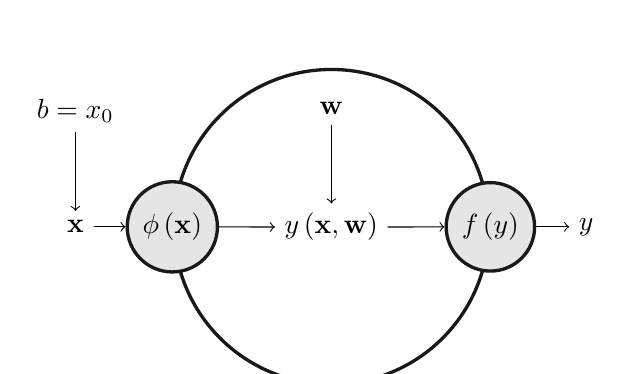
\begin{tikzpicture}[
                    neuron/.style={circle, draw=black!90, very thick},
                    var/.style={}, io/.style={circle, draw=black!90,
                    fill=black!10, very thick, minimum size=7mm},
                ]
                \node (neuron_logic) {$ y\left(\mathbf{x}, \mathbf{w}\right)
                $};
                \node (weights) [above=of neuron_logic] {$ \mathbf{w} $};
                \node[text opacity=0] (invisible) [below=of neuron_logic] {neuron};
                \node[neuron, fit={(weights)(neuron_logic)(invisible)}] (neuron) {};
                % \node[var] (input) [left=of neuron] {$ \mathbf{x} = \begin{bmatrix}x_{0}&x_{1}&\vdot&x_{D}\end{bmatrix} $};
                \node[var] (input) [left=of neuron] {$ \mathbf{x} $};
                \node[var] (bias) [above=of input] {$ b = x_{0} $};
                \node[var] (output) [right=of neuron] {$ y $};
                \node[io] (basis) at (neuron.west) {$
                \mathbf{\phi}\left(\mathbf{x}\right) $};
                \node[io] (activation) at (neuron.east) {$ f\left(y\right) $};

                \draw[->] (bias.south) -- (input.north);
                \draw[->] (input.east) -- (basis.west);
                \draw[->] (basis.east) -- (neuron_logic.west);
                \draw[->] (neuron_logic.east) -- (activation.west);
                \draw[->] (activation.east) -- (output.west);
                \draw[->] (weights.south) -- (neuron_logic.north);
            \end{tikzpicture}
        \end{center}
        \caption{A visual representation of a neuron.}\label{fig:neuron}
    \end{figure}

    Because I couldn't find a simple way of doing anonymous functions in my
    language of choice, \href{run:../src/utils/neural.zig}{my implementation}
    does not allow specifying basis functions nor activation functions so every
    basis function can be thought as being the identify function $
    \mathbf{\phi}(x) = x $ and the activation function can be toggled between
    the identify and sigmoid \eqref{eq:sigmoid}.

    \begin{equation}
        \sigma\left(x\right) = \frac{1}{1+e^{-x}}
        \label{eq:sigmoid}
    \end{equation}

    \section{Feed-Forward Neural Network}

    The idea now, as explained in chapter 5.1 of \cite{bishop}, is to train
    neurons so that their weight values are good.

    Because a neuron is really just a function, a neuron can be a basis
    function of another neuron, starting a network.

    %%% create visual representation of the above

    A network is composed of layers, each with its own number of neurons.

    %%% visual representation of a layer

    Each of neuron will create a value called \textbf{activation} represented
    by $ a_{j} $ \eqref{eq:activation} where $ j $ is the neuron number (we can
    think of a layer as a column matrix of neurons), $ \mathbf{X} $ is the
    function input or the activations from the layer before after they passed
    through an activation function and $ D $ is the amount of row in $
    \mathbf{x} $ $ - 1 $.

    Let's define a way to represent a matrix row:
    $$
        A = \begin{bmatrix}a_{0}\\\vdots\\a_{N}\end{bmatrix} \in \mathbb{R}^{N
            \times M}, a_{i} \in \mathbb{R}^{M}, i \in \left\{ x \in
            \mathbb{N}: x \le N \right\}
    $$
    $$
        A_{i *} = a_{i}
    $$

    \begin{equation}
        \begin{split}
            a_{j} & = f \left( \displaystyle\sum_{i=1}^{D} \left( w_{ji}x_{i}
            \right) + (1)b_{j} \right) \\ & = f \left( \mathbf{x} \cdot W_{j *}
            \right)
        \end{split}
        \label{eq:activation}
    \end{equation}

    The last layer will be the one giving the outputs $ \mathbf{y} $.

    If a neural network has $ n $ layers, the mathematical representation for
    the output $ k $ will be something like \eqref{eq:neural_network}. $
    W^{(n)} $ are the weights of that layer. For this to work, because it's
    just matrix multiplications, we have to be aware of the dimensions of the
    matrixes. This is called \textbf{forward propagation}.

    \begin{equation}
        Y_{0} = \textbf{x}
    \end{equation}
    \begin{equation}
        Y_{n} = f_{n} \left( Y_{n - 1}^{T} \cdot w^{(n)} \right), n > 0
    \end{equation}

    \begin{equation}
        \begin{split}
            y_{k}(\mathbf{x}, \mathbf{w}) & = f_{n} \left( \displaystyle\sum_{i_{n}=0} w_{k i_{n}}^{(n)} \hdots f_{2} \left( \displaystyle\sum_{i_{2}=0} w_{i_{3}i_{2}}^{(2)} f_{1} \left( \displaystyle\sum_{i_{1}=0} w_{i_{2}i_{1}}^{(1)}x_{i_{1}} \right) \right) \hdots \right) = \\
            & = f_{n} \left( \hdots f_{2} \left( f_{1} \left( \mathbf{x} \cdot w^{(1)} \right)^{T} \cdot w^{(2)} \right)^{T} \hdots \cdot w^{(n)} \right) = \\
            & = Y_{n}
        \end{split}
        \label{eq:neural_network}
    \end{equation}

    %%% full conectivity not mandatory

    %%% visual representation of a neural network

    Layers and neural network representation can be found
    \href{run:../src/utils/neural.zig}{\texttt{/src/utils/neural.zig}}.

    %%% create x^2 sin(x) |x|

    \section{Learning}

    Now we can feed our network with some data, and it will give us a response
    (one that we might not want). The network will probably give you some
    nonsense output and that's probably because the weights in each neuron are
    also nonsense.

    Our goal now it's to try and find the optimal weights for the network.

    We will evaluate how bad the network is behaving and after that tell it
    what it should change to do a better job.

    \subsection{Error function}

    First we need a way of measuring how dumb the network is. Error functions
    measures the difference between the network output and the expected output.

    There are a lot of functions that we can choose to calculate that.

    We will use this $ E \left( \mathbf{w} \right) $ error function
    \eqref{eq:error_function} that is a sum of the squares of those differences
    in outputs.

    \begin{equation}
        E_{n} \left( \mathbf{w} \right) = \left| \mathbf{y}(\mathbf{x}_{n}, \mathbf{w}) - \mathbf{t}_{n} \right|^{2}
    \end{equation}

    \begin{equation}
        E \left( \mathbf{w} \right) = \frac{1}{2} \displaystyle\sum_{n=1}^{N} E_{n}(\mathbf{w})
        \label{eq:error_function}
    \end{equation}

    We have the input training matrix $ \left\{ \mathbf{x}_{n} \right\} $, $ N $
    is the input size. Also, we have $ \left\{ \mathbf{t}_{n} \right\} $ with the
    expected outputs for each input.

    Our goal is to minimize the error function \eqref{eq:error_function}
    because the closer to 0 that the error function return gets, means the
    differences between our neural network output and the expected output are
    less big.

    \subsection{Parameter Optimization}

    The way to minimize a function is by calculating its derivative on a point,
    so we can get the instantaneous rate of change at that point, that is, how
    much is the function growing/decreasing on that point. But that only works
    for unary function. Our neural network is a function with an unlimited
    (limited by the hardware which is running on) number of parameters (the
    weights). Because of that we instead use \textbf{partial derivatives}, and
    we calculate it for each one of the neural network weights (and biases if
    they are separated from the weights). Actually, we are calculation what's
    called the \textbf{gradient}, which is a vector of which one of those
    partial derivatives. That vector's direction is towards where that function
    grows (greatest rate of increase), we want to go the other way around.

    Our goal is to reach a minimum with $ \nabla E \left( \mathbf{w} \right) =
    \vec{0} $ and while we don't reach it, we keep changing the weights based
    on $ -\nabla E \left( \mathbf{w} \right) $. One of the problems that might
    arise is that $ \nabla E \left( \mathbf{w} \right) = \vec{0} $ does not
    mean that we found the perfect weight values, because a function can have
    multiple minimums and with the amount of parameters that a neural network
    has, it surely does, but also, it does not mean for sure we meet a minimum
    and instead meet a maximum of saddle point. Also targeting non error can be
    impossible, so we might instead target a maximum error that we allow the
    neural network to have.

    It also probably hard as hell to find the perfect weights only using math;
    I wouldn't get involved in that. At least it would take some time. So
    normally we just give each weight a random value, and we have the initial
    weight vector $ \mathbf{w}^{\left( 0 \right)} $. From that, we iteratively
    update the weights based on a weight vector update $ \Delta
    \mathbf{w}^{\left( \tau \right)} $ as shown in \eqref{eq:weight_updates}.

    \begin{equation}
        \mathbf{w}^{\left( \tau + 1 \right)} = \mathbf{w}^{\left( \tau \right)} + \Delta \mathbf{w}^{\left( \tau \right)}
        \label{eq:weight_updates}
    \end{equation}

    In our case we are going to do \textbf{gradient descent optimization} so
    from \eqref{eq:weight_updates} we get
    \eqref{eq:gradient_descent_optimization}.

    \begin{equation}
        \begin{split}
            \mathbf{w}^{\left( \tau + 1 \right)} & = \mathbf{w}^{\left( \tau \right)} + \Delta \mathbf{w}^{\left( \tau \right)} = \\
            & = \mathbf{w}^{\left( \tau \right)} + \left( \left( \mathbf{w}^{\left( \tau \right)} + \eta \nabla E \left( \mathbf{w}^{\left( \tau \right)} \right) \right) - \mathbf{w}^{\left( \tau \right)} \right) = \\
            & = \mathbf{w}^{\left( \tau \right)} + \eta \nabla E \left( \mathbf{w}^{\left( \tau \right)} \right)
        \end{split}
        \label{eq:gradient_descent_optimization}
    \end{equation}

    The $ \eta > 0 $ and it's called \textbf{learning rate}, so we can define
    how fast we want the optimization to be based on the gradient.

    While implementing this, I had some problems.

    Sometimes the $ E \left( \mathbf{w} \right) $ was minimizing and from out of nowhere it
    would explode into big numbers. But it seems there are some techniques that
    seem to maybe solve that problem such as \textbf{regularization} which is
    mentioned in page 30 \cite{bishop}. It can also be because of the way I
    calculated the derivatives: by using the limit definition. You can define
    an $ \epsilon $ on your neural network, and it will calculate the
    derivatives using it like this: $ \lim_{\epsilon\to\infty} \frac{f(x +
    \epsilon) - f(x)}{\epsilon} $. It would also depend on the input, and the
    initial weights.

    During implementation, I also thought that this system can cause a lot of
    problems in multilayer neural networks, because changing the weights of one
    neuron will affect the behavior of every neuron forward because they depend
    on its activation, and we are changing every weight at the same time.

    But I guess that's why \textbf{error backpropagation} is preferred over
    this method.

    \subsection{Error Backpropagation}

    Maybe because of what I mentioned above, error backpropagation exist, where
    the gradient is calculated from the last layer of the neural network (the
    output layer) to the first.

    This should work for any feed-forward neural network with any activation
    functions and error function.

    We have a general error function which is the sum of the errors of each
    input data.

    \begin{equation}
        E \left( \mathbf{w} \right) = \displaystyle\sum_{n=1}^{N} E_{n}(\mathbf{w})
    \end{equation}

    We want to compute $ \nabla E_{n} \left( \mathbf{w} \right) $.

    So we start by feeding forward where we calculate all the activations for
    every input $ \mathbf{x}_{i} $. In all the equations forward $ \left( \tau
    \right) $ represents the layer.

    Remember from the equation \eqref{eq:linear_model}. Here we have

    \newcommand{\nlayer}{\left( \tau \right)}
    \newcommand{\nplayer}[1]{\left( \tau - {#1} \right)}
    \newcommand{\npblayer}[1]{\left( \tau + {#1} \right)}
    \begin{equation}
        a_{k}^{\nlayer} = \displaystyle\sum_{i} \left( w_{ki}^{\nlayer} z_{i}^{\nplayer{1}} \right)
    \end{equation}

    \begin{equation}
        z_{i}^{\left( \tau \right)} = f^{\left( \tau \right)} \left( a_{i}^{\left( \tau \right)} \right)
    \end{equation}

    \newcommand{\pd}[2]{\frac{\partial {#1}}{\partial {#2}}}
    \newcommand{\ajl}{a_{j^{\nlayer}}^{\nlayer}}
    \newcommand{\ajpl}[1]{a_{j^{\npblayer{#1}}}^{\npblayer{#1}}}
    Now as we did before, we want to calculate the gradient, so we need to
    calculate the partial derivative $ \pd{E_{n}}{w_{ji}^{\nlayer}} $ for every
    weight.

    We can use the derivatives chain rule to write the partial derivative
    because the error function needs the activation after the weight to be
    dependent on that weight.

    \begin{equation}
        \pd{E_{n}}{w_{ji}^{\nlayer}} & = \pd{E_{n}}{a_{j}^{\nlayer}} \pd{a_{j}^{\nlayer}}{w_{ji}^{\nlayer}}
    \end{equation}

    And calculate those two separately.

    \begin{equation}
        \begin{split}
            \pd{E_{n}}{a_{j}^{\nlayer}} & = \pd{}{a_{j}^{\nlayer}} \left( a_{j}^{\left( \tau \right)} - t_{j} \right)^{2} = \\
            & = 2 \left( a_{j}^{\left( \tau \right)} - t_{j} \right) \pd{}{a_{j}^{\nlayer}} \left( a_{j}^{\left( \tau \right)} - t_{j} \right) = \\
            & = 2 \left( a_{j}^{\left( \tau \right)} - t_{j} \right) \left( 1 \right) = \\
            & = 2 \left( a_{j}^{\left( \tau \right)} - t_{j} \right) = \\
            & = \delta_{j}
        \end{split}
    \end{equation}
    \begin{equation}
        \begin{split}
            \pd{a_{j}^{\nlayer}}{w_{ji}^{\nlayer}} & = \pd{}{w_{ji}^{\nlayer}} \displaystyle\sum_{i} \left( w_{ji}^{\nlayer} z_{i}^{\nplayer{1}} \right) = \\
            & = \pd{}{w_{ji}^{\nlayer}} \left( w_{ji}^{\nlayer} z_{i}^{\nplayer{1}} + \displaystyle\sum_{k \neq i} \left( w_{jk}^{\nlayer} z_{k}^{\nplayer{1}} \right) \right) = \\
            & = \left( 1 \right) z_{i}^{\nplayer{1}} + \displaystyle\sum_{k \neq i} 0 = \\
            & = z_{i}^{\nplayer{1}}
        \end{split}
    \end{equation}

    \begin{equation}
        \pd{E_{n}}{w_{ji}} = \delta_{j}^{\nlayer} z_{i}^{\nplayer{1}}
    \end{equation}

    We call $ \delta_{j}^{\nlayer} $ the errors. Because we already calculated
    every $ z_{i}^{\nplayer{1}} $ while forward propagating, we really just
    need to calculate the errors.

    The $ \delta_{j}^{\nlayer} $ we calculated is for the output layer. For the
    layer before that, we can also use the chain rule.

    \begin{equation}
        \begin{split}
            \delta_{j}^{\nplayer{1}} & = \pd{E_{n}}{a_{j}^{\nplayer{1}}} \\
            & = \displaystyle\sum_{k} \left( \pd{E_{n}}{a_{k}^{\nlayer}} \pd{a_{k}^{\nlayer}}{a_{j}^{\nplayer{1}}} \right) = \\
            & = \displaystyle\sum_{k} \left( \delta_{k}^{\nlayer} \pd{}{a_{j}^{\nplayer{1}}} \left( w_{kj}^{\nlayer} f^{\nplayer{1}} \left( a_{j}^{\nplayer{1}} \right) + \displaystyle\sum_{i \neq j} \left( w_{ki}^{\nlayer} z_{ki}^{\nplayer{1}} \right) \right) \right) = \\
            & = \displaystyle\sum_{k} \left( \delta_{k}^{\nlayer} w_{ki}^{\nlayer} f^{\prime \nplayer{1}} \left( a_{i}^{\nplayer{1}} \right)  \right) = \\
            & = f^{\prime \nplayer{1}} \left( a_{j}^{\nplayer{1}} \right) \displaystyle\sum_{k} \left( w_{kj}^{\nlayer} \delta_{k}^{\nlayer} \right)
        \end{split}
    \end{equation}

    \begin{equation}
        \begin{split}
            \pd{E_{n}}{w_{ji}^{\nlayer}} & = \pd{E_{n}}{a_{j}^{\nlayer}} \pd{a_{j}^{\nlayer}}{w_{ji}^{\nlayer}} = \\
            & = \pd{E_{n}}{\ajpl{l}} \displaystyle\prod_{L = 1}^{l} \left( \pd{\ajpl{l - \left( L - 1 \right)}}{\ajpl{l - L}} \right) \pd{\ajl}{w_{ji}^{\nplayer{l}}}
        \end{split}
    \end{equation}

    After calculating all errors from the output layer, you are able to
    calculate from the other layers, one at a time, backwards, and you'll end
    up with the derivatives for the gradient.

    We may also accumulate gradients to apply it to the weights all at once.

    \begin{equation}
        \pd{E}{w_{ji}^{\nlayer}} & = \displaystyle\sum_{n} \pd{E_{n}}{w_{ji}^{\nlayer}}
    \end{equation}

    \medskip

    \printbibliography[
    heading=bibintoc
    ]

\end{document}
